\section{Synthèse et ouverture de l'étude}
\begin{obj}
%Objectif}
Valider le modèle de connaissance, valider la commande optimisée et envisager un prolongement à l'étude.
\end{obj}

\subsection{Validation du modèle de connaissance et de la commande optimisée}%IV.A - 
On appelle commande optimisée la commande avec le correcteur de la boucle d'asservissement de force du type proportionnel avec limitation de la vitesse angulaire. Sur le banc d'essai avec l'actionneur linéaire, on implante ce correcteur, et on procède à quatre essais pour des consignes en échelon de force de $10,20,30$ et 40 N . Les mesures correspondantes sont tracées en traits discontinus sur la figure \ref{ccs_mp_2023_fig_22}. Ce même correcteur est mis en place dans le modèle de connaissance de la figure \ref{ccs_mp_2023_fig_11}, on obtient les réponses temporelles de simulation tracées en traits continus sur la figure \ref{ccs_mp_2023_fig_22}.

%\begin{figure}[h]
%\begin{center}
%  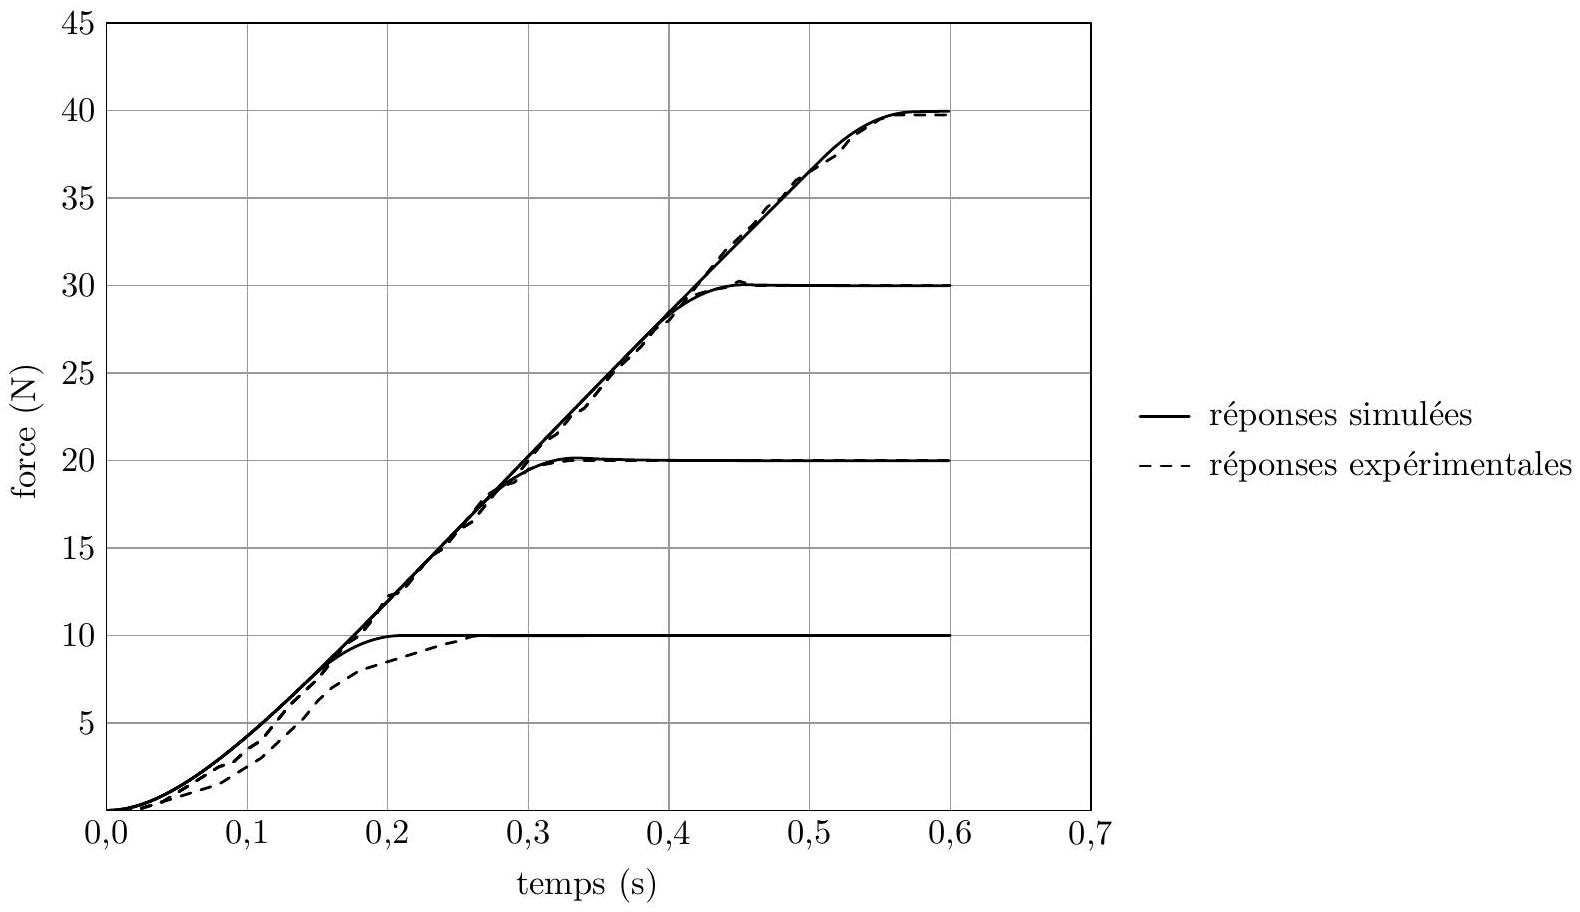
\includegraphics[width=\textwidth]{2025_09_16_5f2d7643f7e649c6833dg-15(1)}
%\captionsetup{labelformat=empty}
%\caption{Figure 22 Résultats des simulations et des expérimentations pour une entrée de consigne de force en échelon d'amplitude 10, 20,30 et 40 N}
%\end{center}
%\end{figure}

\begin{figure}[!h]
\centering
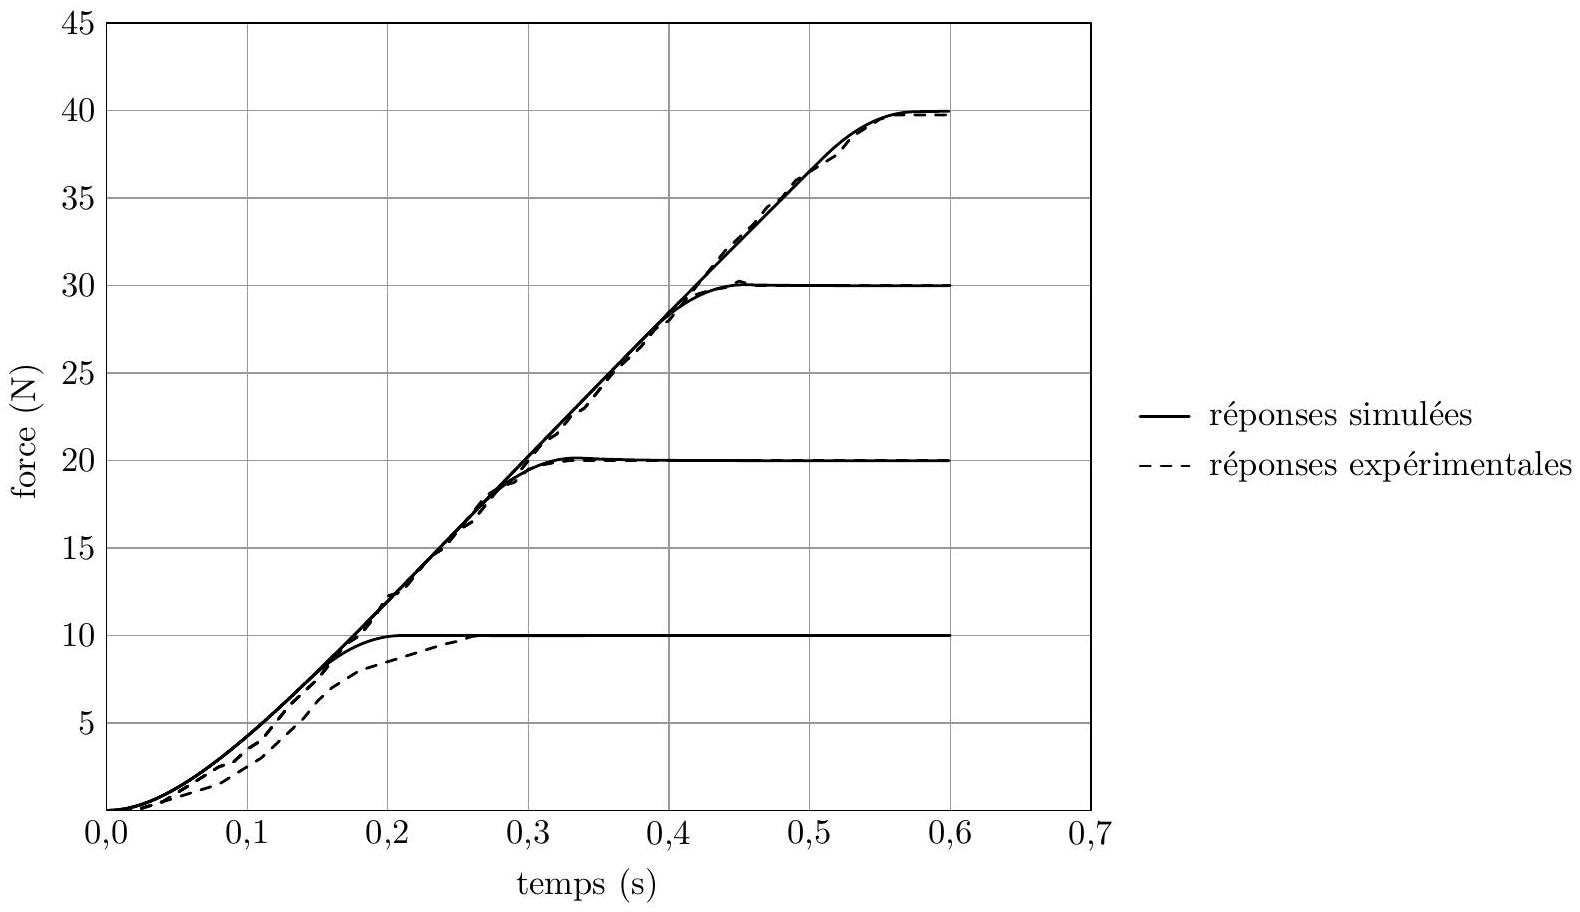
\includegraphics[width=.7\textwidth]{2025_09_16_5f2d7643f7e649c6833dg-15(1)}
\caption{\label{ccs_mp_2023_fig_22}   Résultats des simulations et des expérimentations pour une entrée de consigne de force en échelon d'amplitude 10, 20,30 et \SI{40}{N}}
\end{figure}



La démarche de l'ingénieur abordée dans le programme de sciences industrielles de l'ingénieur de la filière MP s'appuie sur les écarts entre trois performances (figure \ref{ccs_mp_2023_fig_23}).

%\begin{figure}[h]
%\begin{center}
%  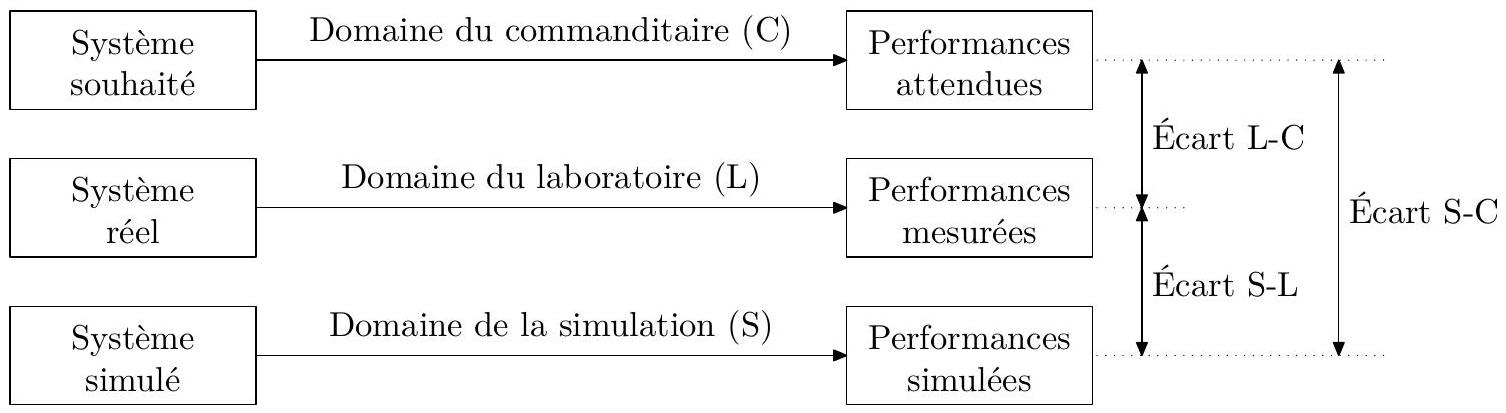
\includegraphics[width=\textwidth]{2025_09_16_5f2d7643f7e649c6833dg-15}
%\captionsetup{labelformat=empty}
%\caption{Figure 23 Synoptique de la démarche de l'ingénieur, telle que présentée dans le programme}
%\end{center}
%\end{figure}


\begin{figure}[!h]
\centering
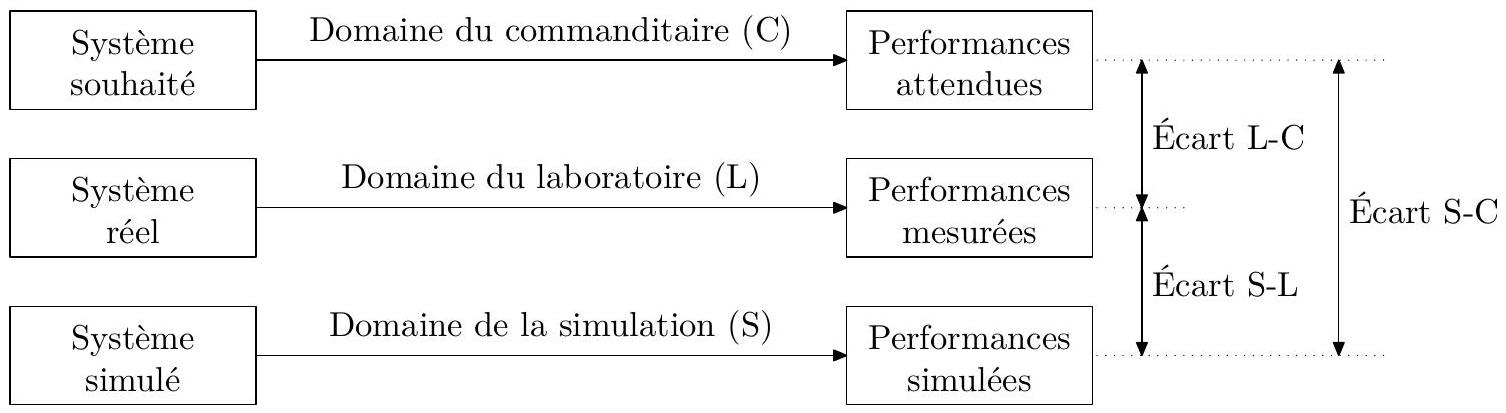
\includegraphics[width=\textwidth]{2025_09_16_5f2d7643f7e649c6833dg-15}
\caption{\label{ccs_mp_2023_fig_23}Synoptique de la démarche de l'ingénieur, telle que présentée dans le programme}
\end{figure}


En se référant à la figure \ref{ccs_mp_2023_fig_22}, l'analyse de l'écart entre les performances simulées et les performances mesurées valide le modèle de connaissance de l'asservissement de force.\\

%Q 29. 
\question{\label{ccs_mp_2023_q_29}
Choisir un des écarts L-C, S-L ou S-C permettant de valider la commande optimisée. Effectuer l'analyse de cet écart. Il est attendu une argumentation rigoureuse s'appuyant sur les données et les références du texte. Les numéros de figure, de tableau, ou d'exigence sont, par exemple, des références utilisables.}
\ifprof
\begin{corrige}
\end{corrige}
\else
\fi


\subsection{Étude du système perturbé}%IV.B - 
Le schéma-blocs de la figure \ref{ccs_mp_2023_fig_24} introduit une perturbation $Y_{\text {pert }}(p)$, représentant une perturbation dans le domaine temporel $y_{\text {pert }}(t)$.

%\begin{figure}[h]
%\begin{center}
%  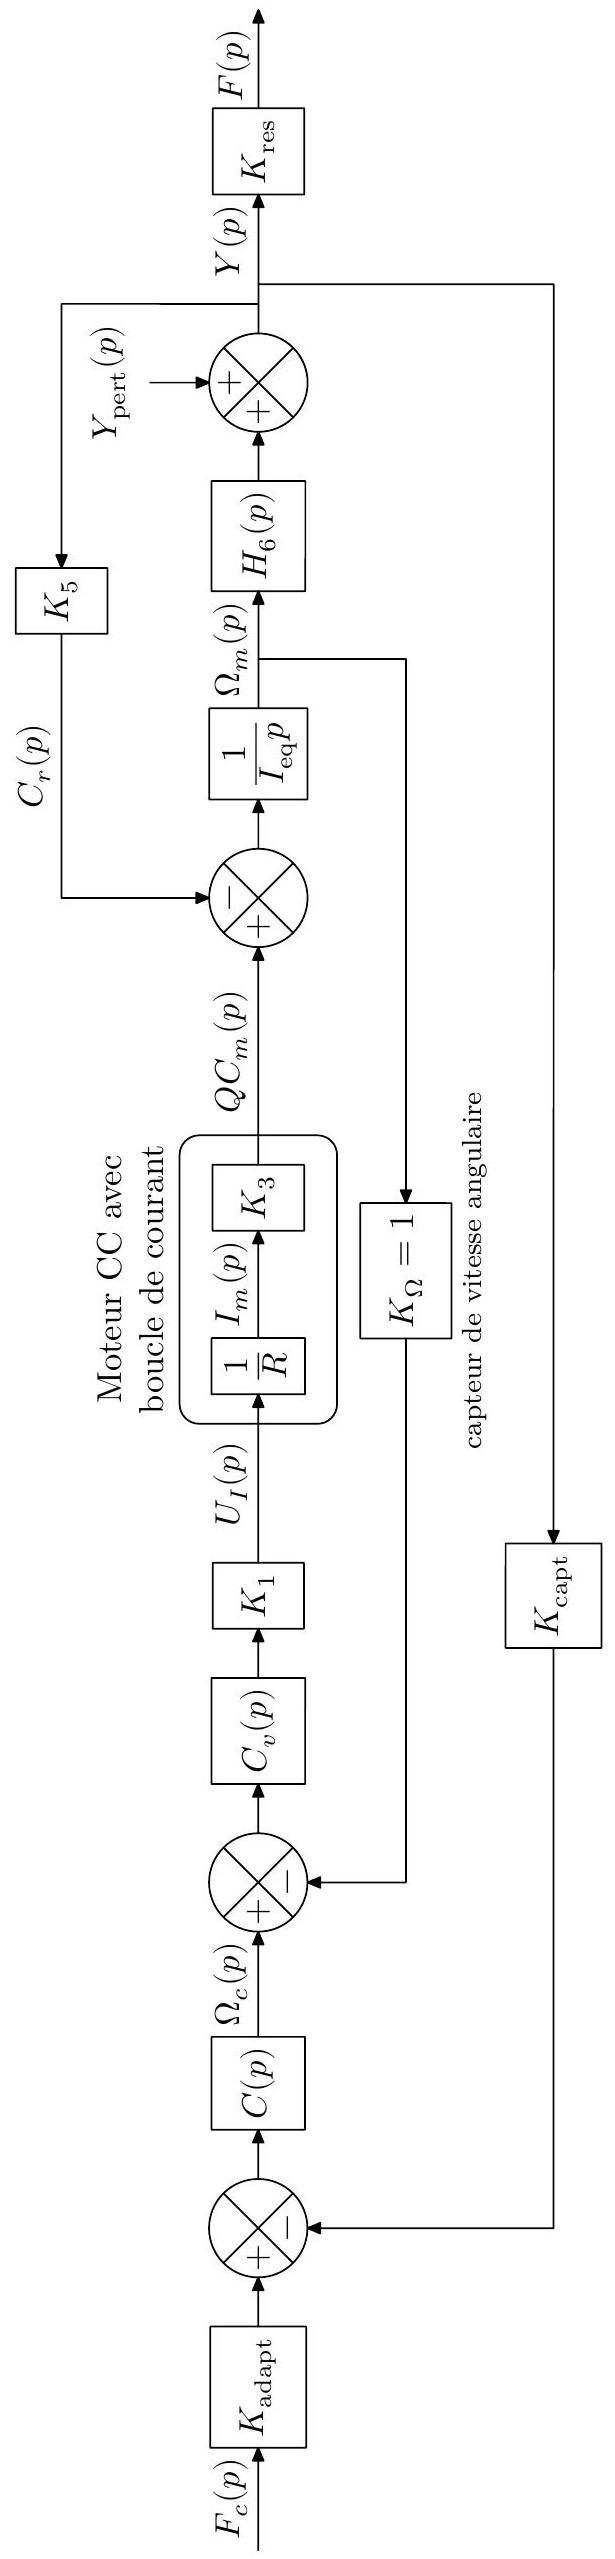
\includegraphics[width=\textwidth]{2025_09_16_5f2d7643f7e649c6833dg-16}
%\captionsetup{labelformat=empty}
%\caption{Figure 24 Schéma-blocs de l'asservissement de force développée par un actionneur linéaire avec perturbation}
%\end{center}
%\end{figure}


\begin{figure}[!h]
\centering
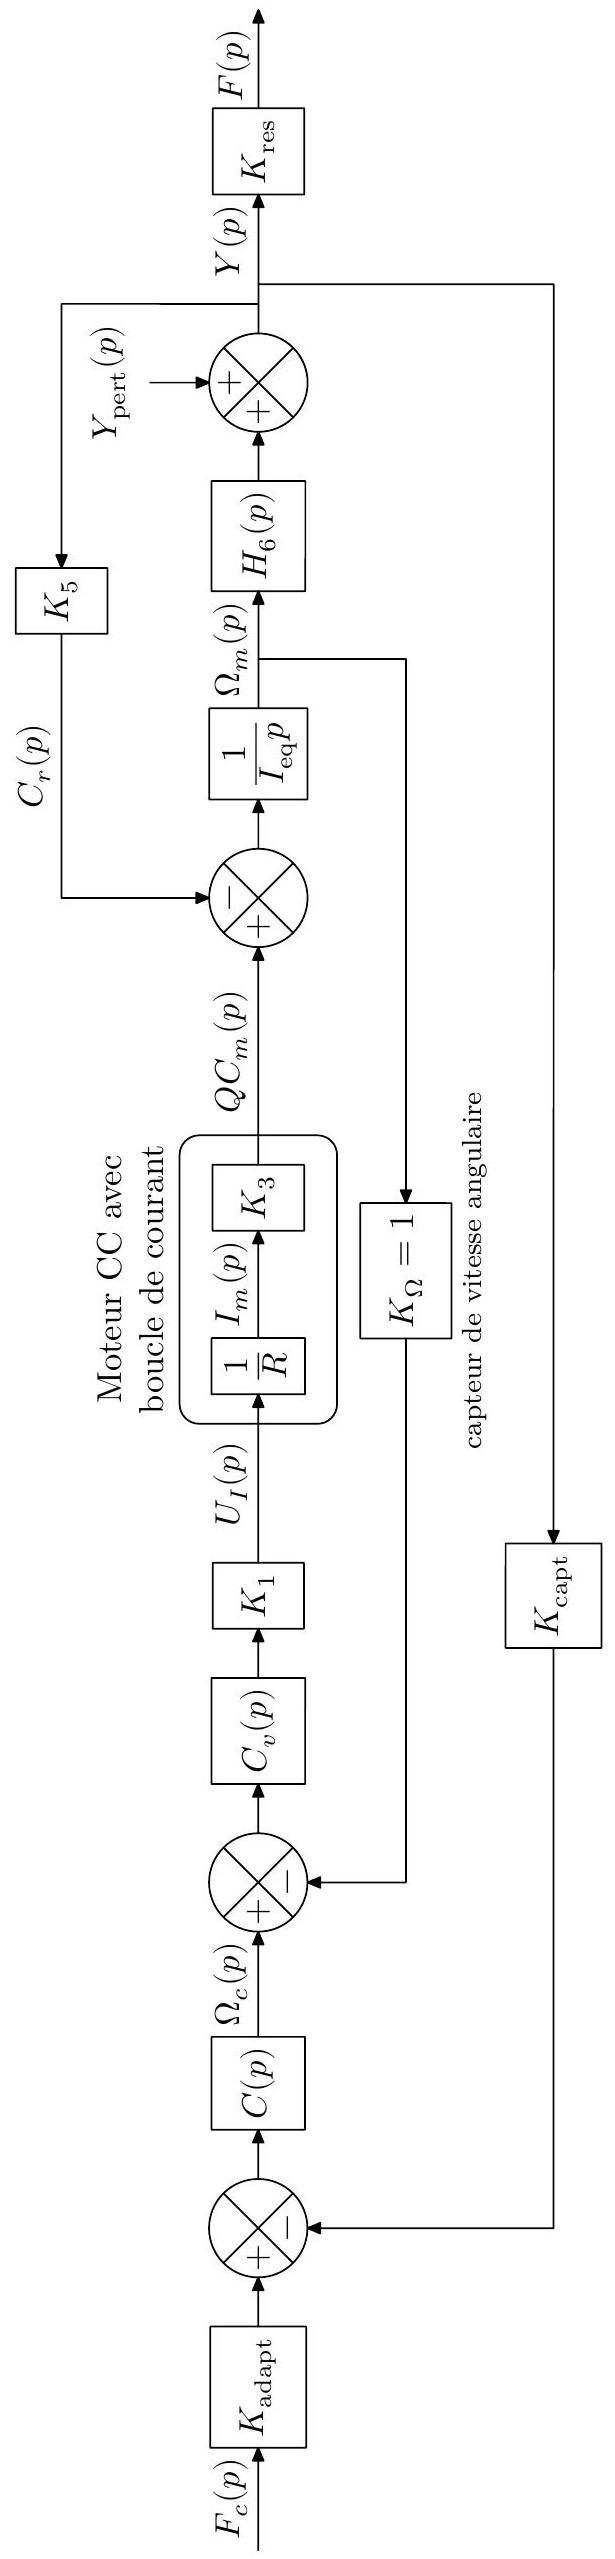
\includegraphics[width=.35\textwidth]{2025_09_16_5f2d7643f7e649c6833dg-16}
\caption{\label{ccs_mp_2023_fig_24}  Schéma-blocs de l'asservissement de force développée par un actionneur linéaire avec perturbation}
\end{figure}

%Q 30. 
\question{\label{ccs_mp_2023_q_30}
Quelle est l'unité de $y_{\text {pert}}(t)$ ? Que peut représenter cette perturbation dans le contexte de l'exosquelette lombaire? En se référant à la problématique du sujet, quel est l'intérêt d'introduire cette perturbation dans le modèle ?}
\ifprof
\begin{corrige}
\end{corrige}
\else
\fi

On effectue une simulation avec une perturbation normalisée représentée sur la figure \ref{ccs_mp_2023_fig_25}.

%\begin{figure}[h]
%\begin{center}
%  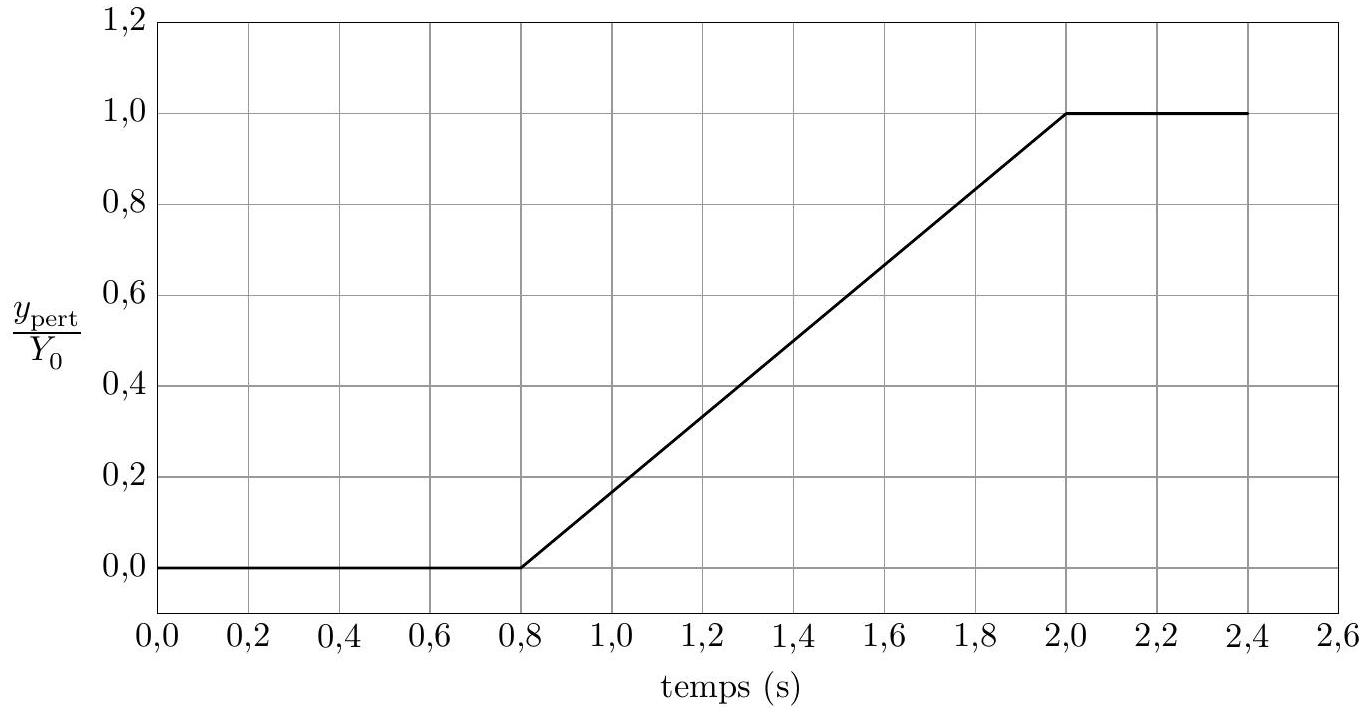
\includegraphics[width=\textwidth]{2025_09_16_5f2d7643f7e649c6833dg-17}
%\captionsetup{labelformat=empty}
%\caption{Figure 25 Évolution temporelle de la perturbation \$y\_\{\textbackslash text \{pert }\}(t)\$\}\end{center}
%\end{figure}

\begin{figure}[!h]
\centering
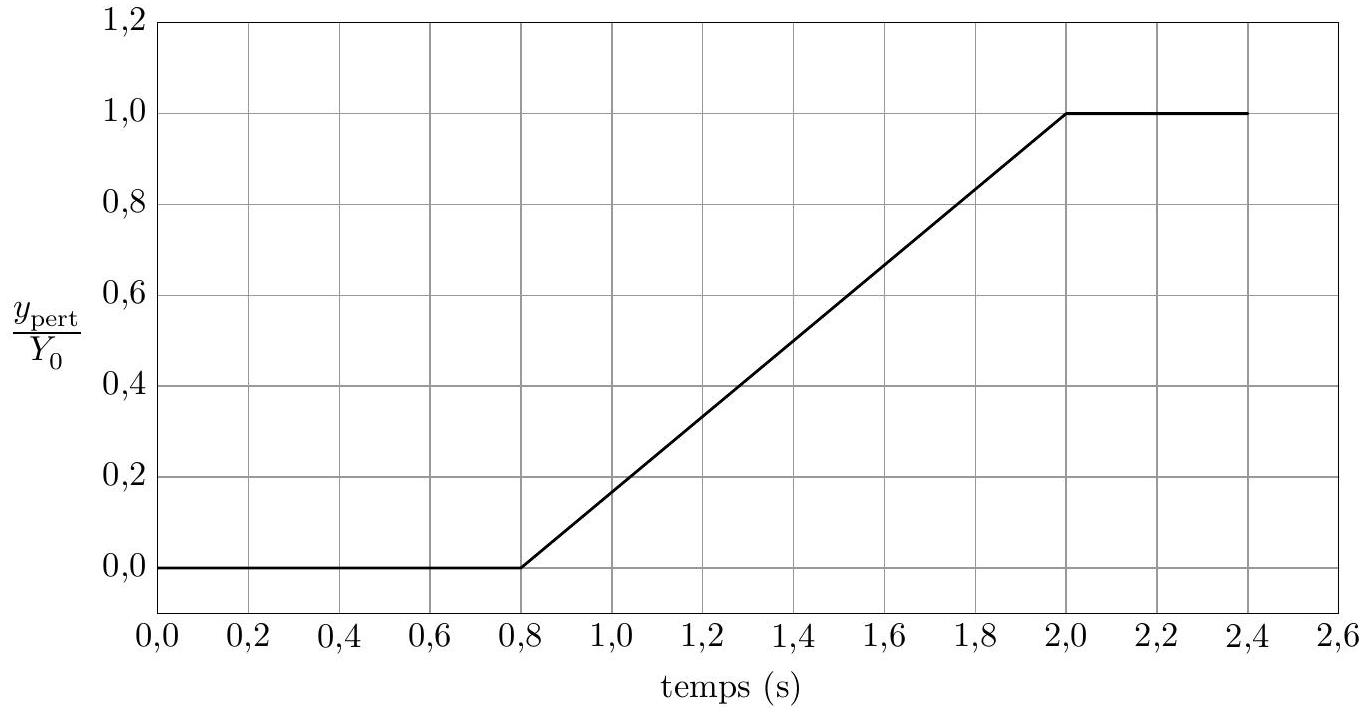
\includegraphics[width=.7\textwidth]{2025_09_16_5f2d7643f7e649c6833dg-17}
\caption{\label{ccs_mp_2023_fig_25}  Évolution temporelle de la perturbation $\indice{y}{pert}(t)$.}

\end{figure}



La figure 26 montre l'évolution de la force développée par un actionneur linéaire soumis à la perturbation décrite sur la figure \ref{ccs_mp_2023_fig_25}. C'est le résultat d'une simulation obtenue à partir du modèle de connaissance avec le correcteur proportionnel et limitation sur la vitesse angulaire.
%
%\begin{figure}[h]
%\begin{center}
%  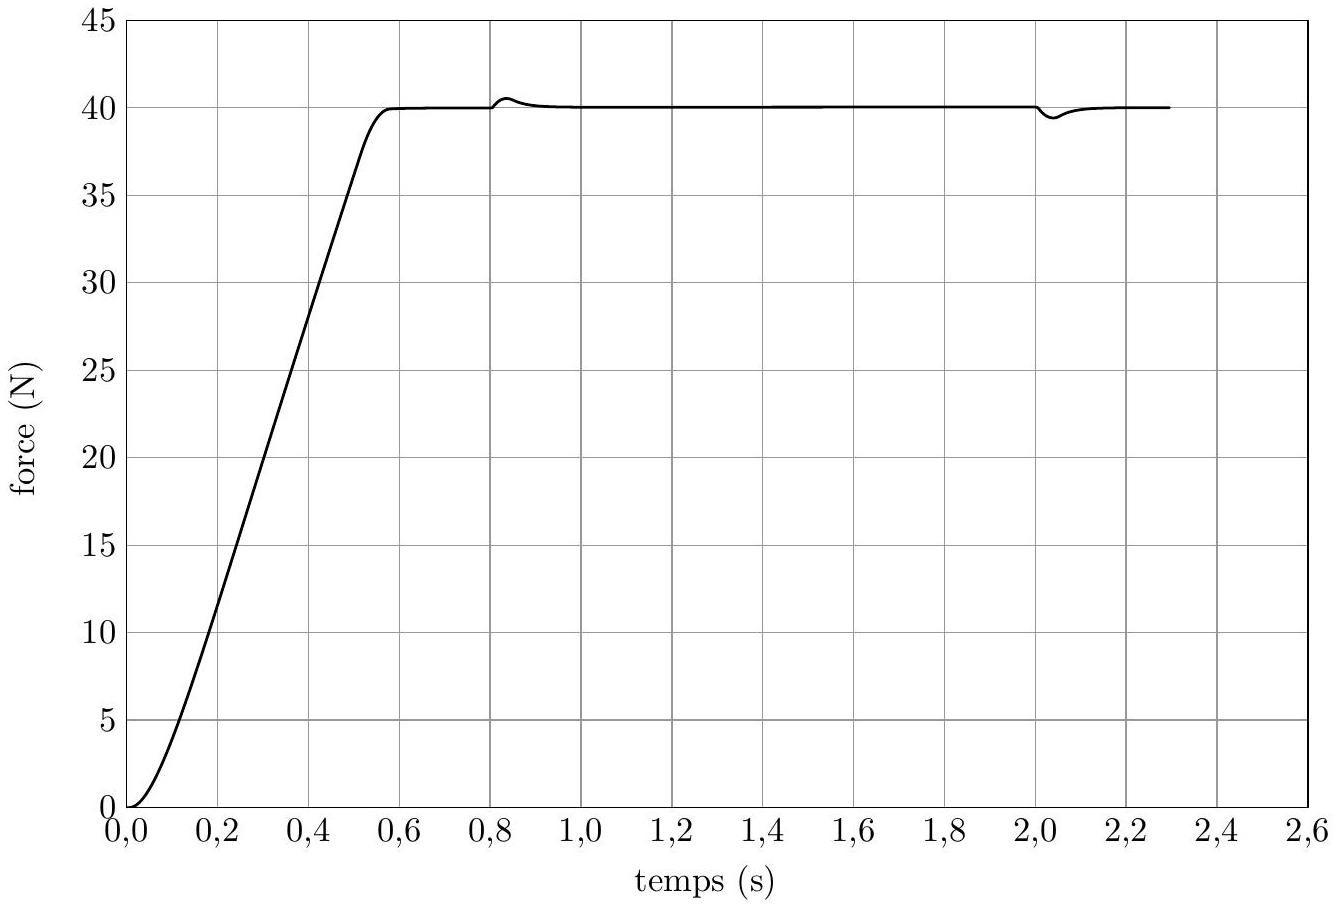
\includegraphics[width=\textwidth]{2025_09_16_5f2d7643f7e649c6833dg-17(1)}
%\captionsetup{labelformat=empty}
%\caption{Figure 26 Évolution de la force développée par l'actionneur linéaire soumis à une perturbation. Consigne en échelon de 40 N avec perturbation à \$t=0,8 \textbackslash mathrm\{\~{}s}\$\}\end{center}
%\end{figure}


\begin{figure}[!h]
\centering
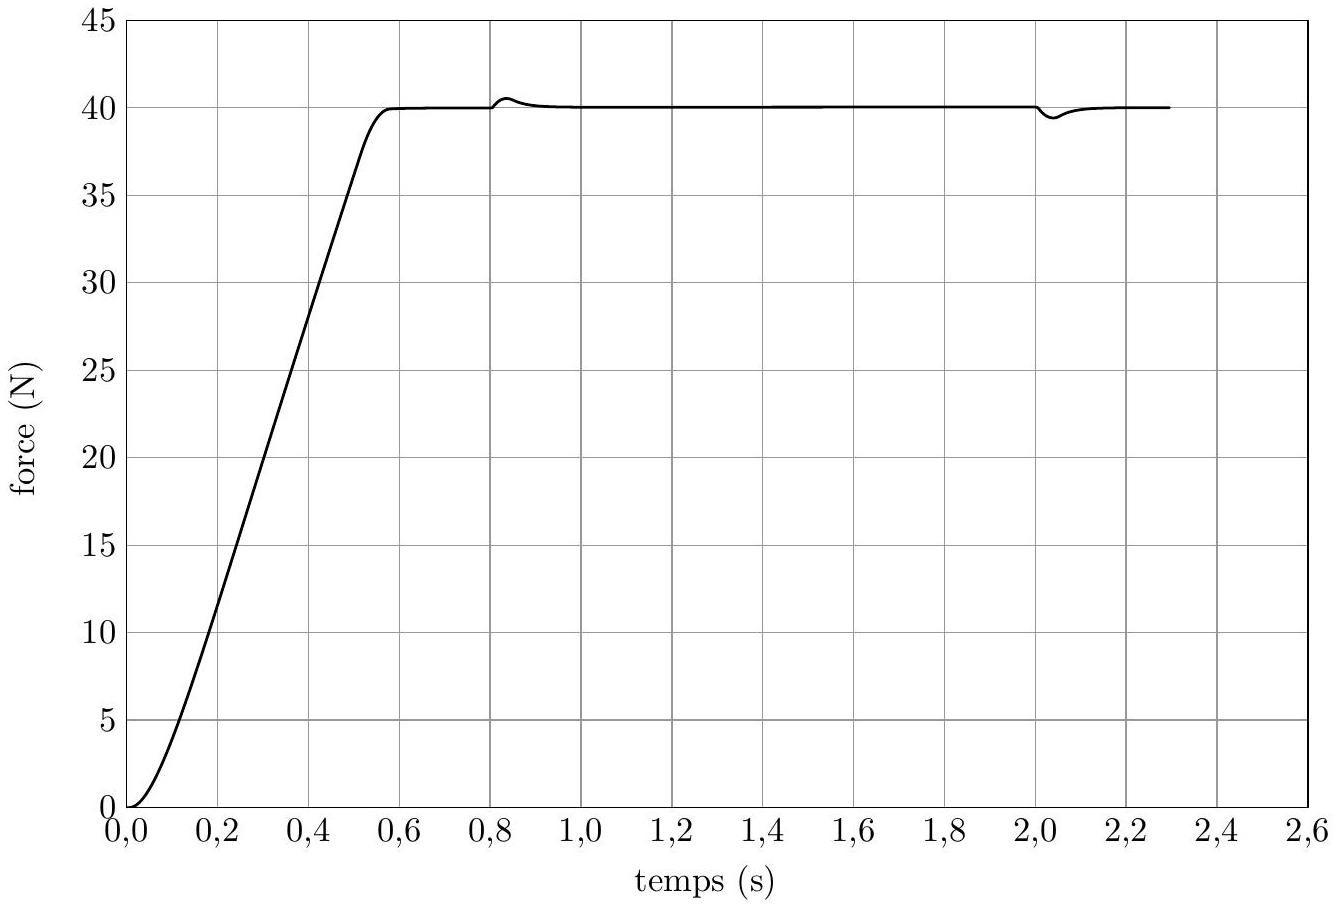
\includegraphics[width=.7\textwidth]{2025_09_16_5f2d7643f7e649c6833dg-17(1)}
\caption{\label{ccs_mp_2023_fig_26}   Évolution de la force développée par l'actionneur linéaire soumis à une perturbation. Consigne en échelon de \SI{40}{N} avec perturbation à $t=\SI{0,8}{s}$.}

\end{figure}



%Q 31. 
\question{\label{ccs_mp_2023_q_31}
Analyser la courbe de simulation de la figure \ref{ccs_mp_2023_fig_26} et conclure au regard de la problématique du sujet.}
\ifprof
\begin{corrige}
\end{corrige}
\else
\fi


%Q 32.
\question{\label{ccs_mp_2023_q_32}
 Le banc d'essai équipé d'un actionneur linéaire, dans la configuration étudiée dans ce sujet, permet-t-il d'analyser l'écart S-L ?}
\ifprof
\begin{corrige}
\end{corrige}
\else
\fi

